\documentclass[12pt]{article}
\usepackage[left=1in,top=1in,right=1in,bottom=1in]{geometry}
\usepackage[font=footnotesize]{caption}
\usepackage{parskip}
\usepackage{times}
\usepackage{graphicx}
\usepackage{mathtools}
\usepackage{gensymb}
\usepackage{placeins}

\setlength{\parskip}{\baselineskip}

\newcommand{\bfvec}[1]{\overline{\mathbf{#1}}}
\newcommand{\spaces}{\phantom{\qquad}}
\newcommand{\under}{\underline{\phantom{\enspace}}}
\newcommand{\diff}{\frac{d}{dt}}

\begin{document}

	\subsubsection*{Simulation}
	
	Source: http://www.myphysicslab.com/runge\_kutta.html
	Source: http://en.wikipedia.org/wiki/List\_of\_Runge\%E2\%80\%93Kutta\_methods
	
	Simulation usually involves integration, for example for an object in free fall. In that case, we have the variables $s$, $v$, $a$, and $t$. The most basic way of implementing integration in a computer program is Euler's method, which is basically choosing a very small time interval $h$ and then incrementing each variable by their derivative multiplied by $h$.

	Say we have a vector $\bfvec{X} = (s, v, a)$, where $\bfvec{X}$ is a vector containing all of the variables in the system. Next, let $\bfvec{X'} = (v, a, 0)$, where $\bfvec{X'}$ is a vector containing the derivative of every variable in the system.

	Suppose that $\bfvec{X}_n$ is the value of the variables at time $t_n$. Then Euler's method is basically
			$$\bfvec{X}_{n+1} = \bfvec{X}_n + \bfvec{X'}_n \cdot h$$
			
	This can be generalized for any system of variables, as specified in the source. Suppose that there are $m$ variables $x_1$, $x_2$, ..., $x_m$, each of which vary over time. In the free fall example, $x_1$ would be position and $x_2$ would be velocity. Suppose there are $m$ differential equations for these $m$ variables
			$$x_1' = f_1(t_n, x_1,x_2,...,x_m)$$
			$$x_2' = f_2(t_n, x_1,x_2,...,x_m)$$
			$$...$$
			$$x_m' = f_m(t_n, x_1,x_2,...,x_m)$$
	Note that there are no derivatives on the right hand side of any of these equations, and that there are only first derivatives on the left hand side. Also, note that each function takes every other variable as an argument even though we don't necessarily need to use every variable. For example, in the free fall example, the derivative of acceleration would just be 0, which is dependent on neither position nor velocity. But for ease of programming, we send all of those variables in as arguments anyway. Rather than cherry-picking which variable this derivative function will require, it's a lot easier to just send all of them and let the function decide which ones to use. 
	
	These equations can be summarized in vector form as
			$$\bfvec{X'} = \bfvec{f}(t_n, \bfvec{X})$$
	where $\bfvec{X} = (x_1,x_2,...,x_m)$ and $\bfvec{f}=(f_1,f_2,...,f_m)$ in a loose "vector of functions" sort of concept. So say we label our time states $\bfvec{X}_n$, $\bfvec{X}_{n+1}$, which are separated by a time interval of length h. Then
			$$\bfvec{X}_n = (x_{1,n}, x_{2,n}, ..., x_{m,n})$$
			$$\bfvec{X}_{n+1} = (x_{1,n+1}, x_{2,n+1}, ..., x_{m,n+1})$$
	So if we have the state of the simulation at time $t_n$ as $\bfvec{X}_n$, we want to compute the state a short time $h$ later and put the results into $\bfvec{X}_{n+1}$. And then do the same for $\bfvec{X}_{n+1}$ and $\bfvec{X}_{n+2}$, and keep going until a stopping condition is reached. This is either the user pressing the exit button on the top right corner of the screen, or some sort of calculated limit that the programmer puts in.

	\subsubsection*{Integration Methods}
	
	We know about Euler's method 
			$$\bfvec{X}_{n+1} = \bfvec{X}_n + \bfvec{X'}_n \cdot h$$
	but we would need a very small time step to achieve any sort of accuracy, and that is computationally expensive. There is a class of integration methods called Runge-Kutta methods, and Euler's method is the simplest of all of them. Euler's method is denoted RK1. Higher order RK methods use things like midpoint rule or Simpson's rule to achieve higher accuracy for larger time intervals. For example, RK4, or ``\textit{the} Runge-Kutta method'', does the following:
			$$\bfvec{a}_n = \bfvec{f}(t_n, \bfvec{X}_n)$$
			$$\bfvec{b}_n = \bfvec{f}(t_n + \frac{h}{2},\bfvec{X}_n + \frac{h}{2}\ \bfvec{a}_n)$$
			$$\bfvec{c}_n = \bfvec{f}(t_n + \frac{h}{2},\bfvec{X}_n + \frac{h}{2}\ \bfvec{b}_n)$$
			$$\bfvec{d}_n = \bfvec{f}(t_n + h, \bfvec{X}_n + h\ \bfvec{c}_n)$$
			$$\bfvec{X}_{n+1} = \bfvec{X}_n + \frac{h}{6}\ (\bfvec{a}_n + 2\ \bfvec{b}_n + 2\ \bfvec{c}_n + \bfvec{d}_n)$$
			
	A general Runge-Kutta method can be specified using a Butcher tableau, which is of the form	
			\[\begin{array}{c|cccc}
				c_1    & a_{11} & a_{12}& \dots & a_{1s}\\
				c_2    & a_{21} & a_{22}& \dots & a_{2s}\\
				\vdots & \vdots & \vdots& \ddots& \vdots\\
				c_s    & a_{s1} & a_{s2}& \dots & a_{ss} \\
				\hline
       			& b_1    & b_2   & \dots & b_s\\
			\end{array}\]
	The Runge-Kutta method for that particular Butcher tableau is defined as follows:
			$$\bfvec{X}_{n+1} = \bfvec{X}_n + h \sum_{i=1}^s b_i k_i$$
			$$k_i = \bfvec{f}\left(t_n + c_i h, \bfvec{X}_n + h \sum_{j = 1}^{s} a_{ij} k_j\right)$$

	In the solenoid simulator, $t$ is not time but rather some parameter, but the general concept is the same. The program can only use RK1, RK2 or RK4 because we couldn't find the Butcher tableau for any higher order RK methods. The Butcher tableau for the RK1 method that we used is:
			\[\begin{array}{c|c}
				0 & 0 \\
				\hline
  				  & 1 \\
			\end{array}\]			
	The Butcher tableau for the RK2 method that we used is:	
			\[\begin{array}{c|cc}
				0   & 0   & 0  \\
				1/2 & 1/2 & 0  \\
				\hline
    				& 0   & 1  \\
			\end{array}\]			
	The Butcher tableau for the RK4 method that we used is:
			\[\begin{array}{c|cccc}
				0   & 0   & 0   & 0   & 0\\
				1/2 & 1/2 & 0   & 0   & 0\\
				1/2 & 0   & 1/2 & 0   & 0\\
				1   & 0   & 0   & 1   & 0\\
				\hline
    				& 1/6 & 1/3 & 1/3 & 1/6\\
			\end{array}\]
	The RK1 is a first order method, called the ``Forward Euler''. It lacks stability, which means any error introduced accumulates in a positive feedback loop. It also has significant accuracy limits, so it is not an ideal integration method if any accuracy is desired.
	
	The RK2 is a second order method, called the ``Explicit midpoint method''. It is significantly more accurate than RK1. 
	
	The RK4 is a fourth order method; the ``original'' Runge-Kutta method. It is more accurate than RK2.
	
	Both RK2 and RK4 algorithms exhibit elements of numerical stability, which is good because then any errors introduced in the numerical integration tend to be damped out. The effect of a higher-order RK method is basically to provide the same level of accuracy for a smaller number of time intervals, which reduces computational cost. 
	
	\subsubsection*{Magnetism}
	
	Okay, about that $t$ not being time business. See, we want to know the magnetic field of a particular system of wires and current in 3-space in one particular moment in time. Obviously in real life, this field would then induce emfs in the wires and then change the state of the wires which would then change the magnetic and electric fields and ugh that's too complicated. Our simulation is going to have solenoids floating in space not connected to a power source, so obviously it's not going to be accurate in that sense.
	
	We are only concerned with $\vec{B}$ at this instant in time. So remember, $t$ is not time. It is a parameter. This is useful because our wires are 1D functions in 3D, so the x,y,z coordinates can be computed as a function of this single argument (a.k.a. parameter). ``Regrettably, the variable $t$ is often chosen to represent the parameter. One must remember that this has nothing to do with time!''(van Bemmel, 04 September 2014). In our case, it is rather fortunate that the parameter is $t$ because that means we don't have to change notation (lazy).
	
	First principles time. From Mr. van Bemmel's biosavart primer, the law of Biot-Savart describes the differential magnetic field due to a current element by:
	
			$$d\vec{B} = \frac{\mu_0}{4\pi} \, \frac{i\,d\vec{s} \times \vec{r}}{r^3}$$			
	Where: \\
		\spaces $d\vec{B}$ = the differential magnetic field at one specific reference point (T) \\
		\spaces $\mu_0 =$ the permeability constant = 4$\pi \times 10^{-7}$ TmA$^{-1}$ exactly \\		
		\spaces $i$ = the current in the current element (A) \\
		\spaces $d\vec{s}$ = the differential displacement in the current element (m) \\
		\spaces $\vec{r}$ = the position vector pointing from the current element to the reference point \\
		\spaces $r$ = the distance between the current element and the reference point (m)\\
		
	To determine the $\vec{B}$ at a specific reference point, we sum all of these little $d\vec{B}$'s along the wire. Thus, the general algorithm is this: For each reference point, find the numerical integral $d\vec{B}$ along each wire and sum these together to get the $\vec{b}$ at that point.
	
	To compute this integral, we need the following variables: \\
		\spaces 1. $\vec{P}$ - the position of the reference point (m)\\
		\spaces 2. $\vec{s}$ - the position on the wire (m)\\
		\spaces 3. $\vec{B}$ - the magnetic field at the reference point (T)
		
	We don't really need $\vec{r}$ since it can easily be computed from $\vec{P} - \vec{s}$. If we parameterize these variables with the parameter $t$, then
			$$\vec{P}_0 = (P_x, P_y, P_z)$$
			$$\vec{s}_0 = \text{get\under s}(0)$$
			$$\vec{B}_0 = (0, 0, 0)$$
	We choose $\vec{P}$, and we begin $\vec{B}$ with the additive identity, the zero vector. We will denote the position on the wire with the function get\under(0) now, as this is dependent on the geometry of the wire. We will get more into that later. Next, finding the derivatives with respect to t, we have:
			$$\diff \vec{P} = (0, 0, 0)$$
			$$\diff \vec{s} = \text{diff\under s}(t)$$
			$$\diff \vec{B} = \frac{\mu_0}{4\pi} \, \frac{i\,\diff \vec{s} \times \left(\vec{P} - \vec{s}\right)}{|\vec{P} - \vec{s}|^3}$$			
	 	 
	
		

		%\begin{figure}[ht!] 
		%\centering
		%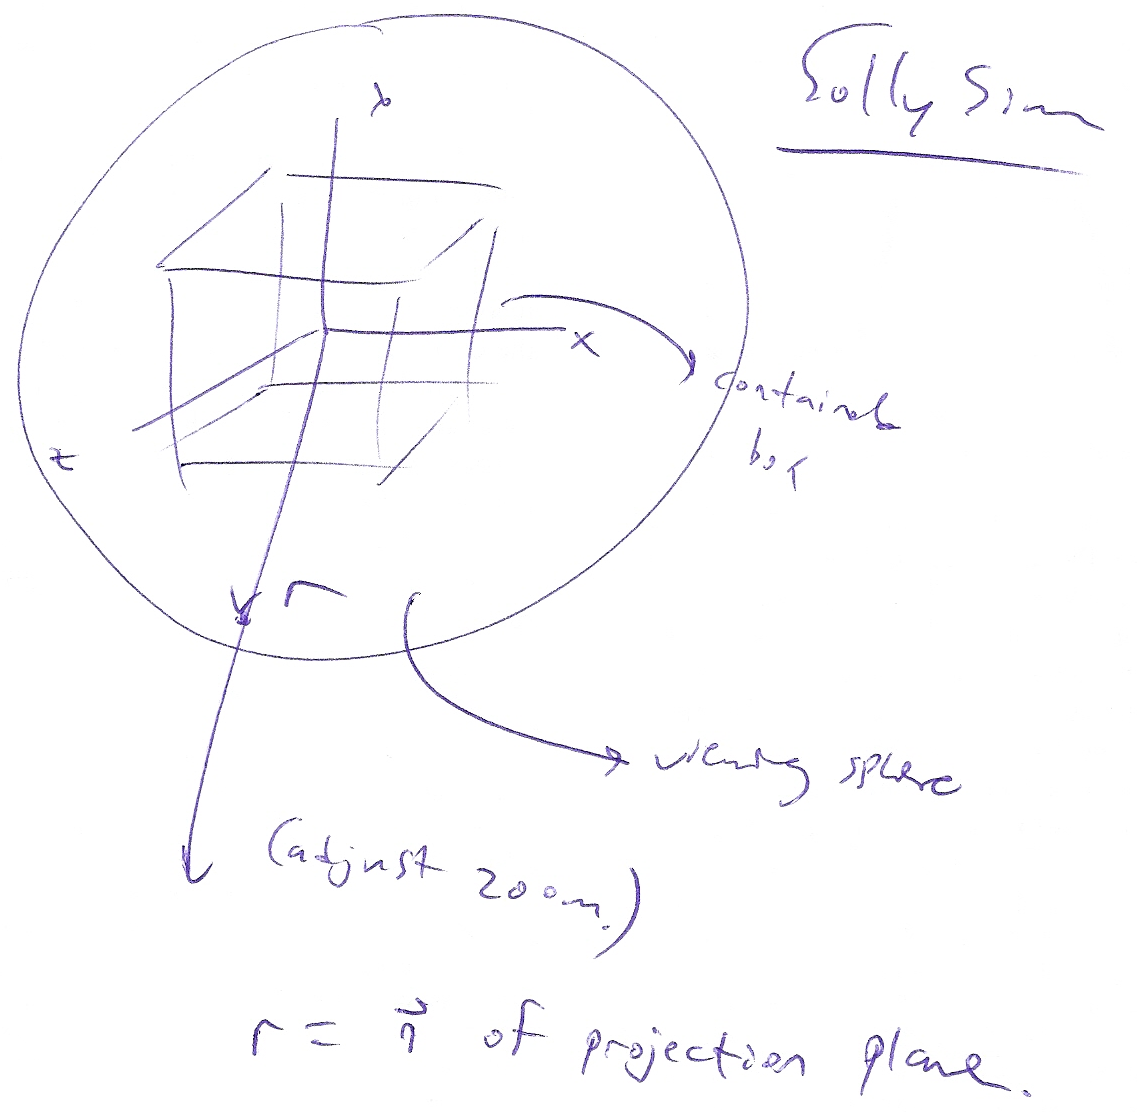
\includegraphics[width=10cm]{1.png}
		%\caption{Our point of view can be anywhere on this sphere, looking in towards the origin. The image will be projected onto a plane normal to this sphere. The resulting image can be scaled afterwards to adjust zoom.} \label{im:1}		
		%\end{figure}

\end{document}